\chapter{Sobre la empresa}

	\section{Historia de Movalsys S.L.}
	
		Movalsys nace como empresa en diciembre de 2015, fruto del ejercicio de estudio y análisis de dos grupos de investigación de la Universidad Pública de Navarra, el grupo de \textit{"Álgebra y Aplicaciones"} y el de \textit{"Biomecánica y Fisiología del movimiento, BIOFIM"}. 
		
		La actividad de Movalsys S.L. consiste en desarrollar y comercializar tecnología para caracterizar el movimiento humano, a través de la obtención de parámetros biomecánicos. Esta caracterización se muestra al usuario de manera simple y directa, para facilitar la interpretación del estado físico de este y su rendimiento. Esto es posible gracias al conocimiento reunido durante más de una década por investigadores de la Universidad Pública de Navarra en la materia. 
		
		El objetivo de la empresa es ofrecer a los profesionales sanitarios una herramienta de trabajo que les permita dar un servicio mejor a sus pacientes. Sirviendo el producto de Movalsys S.L. como apoyo en el diagnóstico y seguimiento de la evolución del paciente. Ayudando a mejorar el proceso de rehabilitación del paciente en casos de rehabilitación, o evaluar la condición física del usuario en casos de medición deportiva. Todo ello al facilitar al cliente el acceso a las métricas biomecánicas del movimiento humano.
		

	\section{Dedicación de la empresa}
	
		El equipo de Movalsys S.L. lleva ocho años realizando investigaciones sobre el análisis de señales biomecánicas proporcionadas por sensores inerciales. Sus avances han sido publicados en importantes revistas científicas en Fisioterapia, Geriatría, Ingeniería y Matemáticas.
		
		La empresa se dedica fundamentalmente a desarrollar el software necesario para procesar parámetros obtenidos de sensores inerciales, a fin de analizar el movimiento del cuerpo humano. Así pues su campo de aplicación es amplio, desde la mejora de rendimiento y prevención de lesiones en el campo deportivo, hasta la prevención de caídas y diagnóstico del nivel de fragilidad en el campo geriátrico. En la figura 2.1 se representan los sectores de clientes de la empresa.
		
	 \begin{figure}[H]
	 	\centering
	 	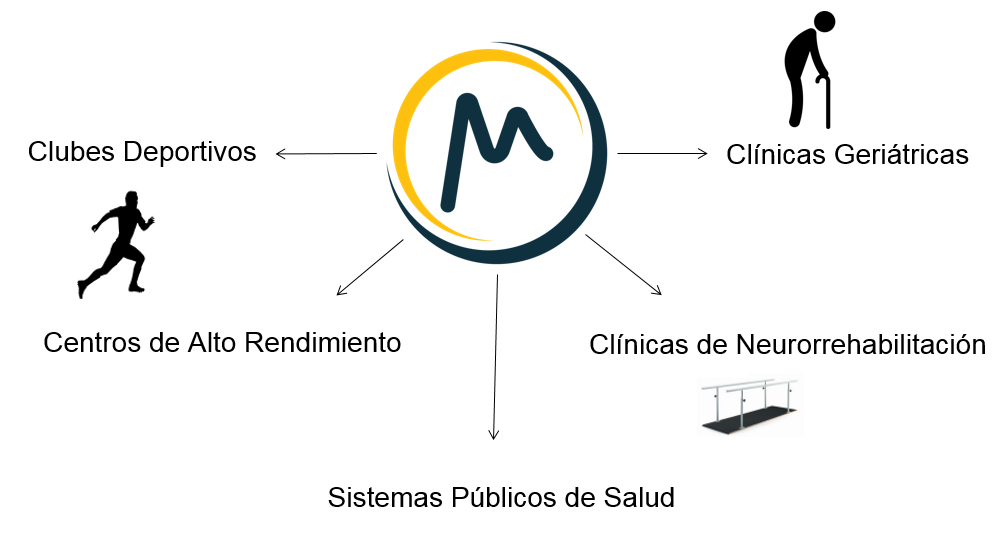
\includegraphics[width=0.8\textwidth]{./graphics/mercado}\label{mercado}
	  	\caption{Sectores de clientes de la empresa.} 
	 \label{fig:mercado}
	 	
	 \end{figure}
 
	\section{Estructura de la empresa} \label{empresa}
	

		Movalsys S.L. es una sociedad limitada donde todos sus trabajadores son socios de esta. Contando además con colaboración externa en el desarrollo de su actividad. 
		
		En el resto del apartado se presenta a cada uno de los integrantes del equipo durante las prácticas y sus funciones dentro de la empresa:
		
		
		\begin{itemize}
			
			\begin{figure}[H]
				\centering
				{\large \textbf{Mariano Velasco}\\}\smallskip
				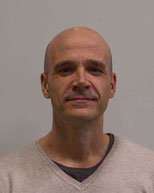
\includegraphics[width=0.25\textwidth]{./graphics/mariano}	
			\end{figure}			
			\item Mariano es el director gerente. Su cometido principal es la gestión de la empresa, tanto de coordinar el equipo como de los asuntos burocráticos. Se encarga además de reunirse con miembros de otras empresas para conseguir proyectos, así como de dar a conocer la empresa asistiendo a diversos eventos. Es la imagen pública de la empresa.  \\
			\bigskip
			
			
			\begin{figure}[H]
				\centering
				{\large \textbf{Pablo Lecumberri}\\}\smallskip
				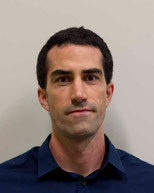
\includegraphics[width=0.25\textwidth]{./graphics/pablo}	
			\end{figure}
			
			\item Pablo es ingeniero de software. Se encarga de la programación del software de medición que utiliza la empresa. En las reuniones con los clientes cumpe un papel técnico crucial para transmitir la viabilidad técnica de las sugerencias de los clientes. \\
			\bigskip
			
			
			
			\begin{figure}[H]
				\centering
				{\large \textbf{Marisol Gómez}\\}\smallskip
				
\includegraphics[width=0.25\textwidth]{./graphics/marisol}	
			\end{figure}
			\item Marisol es directora de investigación. Es la encargada de buscar nuevas convocatorias de ayudas a investigación para empresas, además de ser la encargada de conocer a las incorporaciones a la empresa en puestos de prácticas. Además, busca nuevas áreas de desarrollo a las que se pueda dedicar la empresa. \\ 
			\bigskip
			
			\begin{figure}[H]
				\centering
				{\large \textbf{Alicia Martínez}\\}\smallskip
				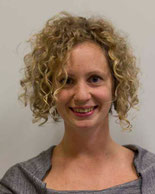
\includegraphics[width=0.25\textwidth]{./graphics/alicia}	
			\end{figure}
			\item Alicia es la responsable de ventas. Se encarga de la gestión de facturas así como de la búsqueda de nuevos clientes. \\
			\bigskip
			
			\begin{figure}[H]
				\centering
				{\large \textbf{Nora Millor}\\}\smallskip
				\includegraphics[width=0.25\textwidth]{./graphics/Nora}	
			\end{figure}
			\item Nora es la responsable de atención al cliente. Es al encargada de estar en contacto con clientes, realizar un seguimiento de funcionamiento del sistema y de mantener las redes sociales. \\
			\bigskip
			
			
			\begin{figure}[H]
				\centering
				{\large \textbf{Mikel Izquierdo}\\}\smallskip
				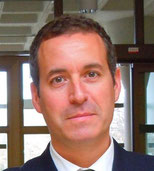
\includegraphics[width=0.25\textwidth]{./graphics/mikel}	
			\end{figure}
			\item Mikel es catedrático y director del departamento de Ciencias de la Salud. Se trata de un profesional muy reconocido en el campo de la salud y por ello también actúa como asesor y se dedica además a la búsqueda de contactos.\\
			\bigskip
			
			\begin{figure}[H]
				\centering
				{\large \textbf{Patxi Iriarte}\\}\smallskip
				
\includegraphics[width=0.25\textwidth]{./graphics/patxii}	
			\end{figure}
			\item Patxi es un estudiante del grado en Ingeniería Informática en la Universidad Pública de Navarra que se encuentra realizando las practicas curriculares. Se dedica al desarrollo software para mejorar las prestaciones este.\\
			\bigskip
			
			
			\begin{figure}[H]
				\centering
				{\large \textbf{Martín Leturia}\\}\smallskip
				
\includegraphics[width=0.25\textwidth]{./graphics/martin}	
			\end{figure}
			\item Martín es un estudiante del grado en Ingeniería de Diseño Industrial y Desarrollo de Producto en la Universidad de Navarra (Tecnun) que ha empezado prácticas en la empresa. Se dedica al diseño de producto.
			\bigskip
			
			
			\begin{figure}[H]
				\centering
				{\large \textbf{Igor Setuain}\\}\smallskip
				
			\end{figure}
			\item Igor es un colaborador externo. Es doctor en fisioterapia, trabaja actualmente en la recuperación funcional de deportistas de Navarra y comunidades limítrofes.\\
			
		\end{itemize}
		\bigskip
	
	Aunque cada miembro del equipo tenga unos cometidos específicos asignados, existen ciertas tareas (por ejemplo: darse a conocer y relacionarse con el cliente) en las que en mayor o menor medida todos participan.
	
	En cuanto a la toma de decisiones, aunque la decisión final recaiga sobre una persona, se tienen en cuenta las opiniones y consideraciones del resto del equipo. Este tipo de conversaciones se dan sobretodo en las reuniones de empresa que se celebran semanalmente. Esta práctica favorece las consecuencias de las decisiones tomadas, además de generar un sentimiento de pertenencia y responsabilidad a los trabajadores, tanto a los trabajadores en prácticas cómo a los trabajadores socios. 

	\section{Plan estratégico}
	
	Movalsys S.L. es una start-up debido al modelo de negocio que tiene y una pyme por el número de empleados que la compone. 
	
	Por su característica de start-up no existe un plan estratégico claro. La falta de ello caracteriza precisamente este tipo de empresas, que aún no se encuentran en la fase madura de empresa.
	
	Por lo tanto, tiene gran importancia la actividad de búsqueda de producto y clientes/proyectos. Durante estos últimos meses se ha ido estableciendo en la empresa lo que podría ser un modelo de negocio más definido, con el nuevo producto \textit{Jero}.

	Además de la experiencia en el campo de aplicación mencionado al principio del documento, en la empresa se cuenta ya con una experiencia de rodaje en cuanto a la relación con el cliente, las tomas de decisiones y nuevas propuestas entrantes.

		
	
	\section{Funcionamiento general}
	
	El funcionamiento de la empresa es bastante presumible, cada empleado tiene claro su cometido fundamental, y se dedica e él, ayudando en el resto de tareas cuando es necesario. 
	
	En general, en una semana en Movalsys S.L. se celebran reuniones con clientes y se desarrollan los proyectos que están en marcha. Además, se celebra una reunión semanal de equipo y un seminario cada dos semanas.
	
	El ambiente de trabajo es muy bueno. La única pena es la falta de personal para poder repartir la carga de trabajo o reducir el tiempo de desarrollo. El compañerismo es una cualidad presente en todo el equipo, siempre hay alguien dispuesto a prestar ayuda. Entrar en un equipo así genera un sentimiento de pertenencia que es fuente de motivación para trabajar. El hecho de ser una empresa pequeña con los roles poco aislados ayuda a aprender en diversos campos.
	
	
	